% This file was created with tikzplotlib v0.10.1.
\begin{tikzpicture}

\definecolor{darkorange25512714}{RGB}{255,127,14}
\definecolor{darkslategray38}{RGB}{38,38,38}
\definecolor{lightgray204}{RGB}{204,204,204}
\definecolor{steelblue31119180}{RGB}{31,119,180}

\begin{axis}[
axis line style={lightgray204},
height=0.375\textheight,
legend cell align={left},
legend style={
  fill opacity=0.8,
  draw opacity=1,
  text opacity=1,
  at={(0.03,0.97)},
  anchor=north west,
  % draw=none
},
tick align=outside,
tick pos=left,
title={Serial Implementation Comparison},
width=\textwidth,
x grid style={lightgray204},
xlabel=\textcolor{darkslategray38}{Mesh size},
xmajorgrids,
xmin=-300000, xmax=28300000,
xtick style={color=darkslategray38},
xtick={-5000000,0,5000000,10000000,15000000,20000000,25000000,30000000},
xticklabels={\ensuremath{-}0.5,0.0,0.5,1.0,1.5,2.0,2.5,3.0},
y grid style={lightgray204},
ylabel=\textcolor{darkslategray38}{Total time (s)},
ymajorgrids,
ymin=-4.88467607640496, ymax=216.204185900316,
ytick style={color=darkslategray38}
]
\path [draw=black, semithick]
(axis cs:1000000,5.16481764980962)
--(axis cs:1000000,5.63830735019038);

\path [draw=black, semithick]
(axis cs:3375000,19.113269268153)
--(axis cs:3375000,19.198180731847);

\path [draw=black, semithick]
(axis cs:8000000,45.0572061385652)
--(axis cs:8000000,46.2580438614348);

\path [draw=black, semithick]
(axis cs:15625000,84.9558151201549)
--(axis cs:15625000,88.3661348798451);

\path [draw=black, semithick]
(axis cs:27000000,144.202737917063)
--(axis cs:27000000,154.023762082937);

\path [draw=black, semithick]
(axis cs:1000000,6.85489901375067)
--(axis cs:1000000,7.18950098624933);

\path [draw=black, semithick]
(axis cs:3375000,22.1573131184878)
--(axis cs:3375000,23.3257368815122);

\path [draw=black, semithick]
(axis cs:8000000,60.0949440654008)
--(axis cs:8000000,61.7840559345992);

\path [draw=black, semithick]
(axis cs:15625000,118.342476046812)
--(axis cs:15625000,120.701023953188);

\path [draw=black, semithick]
(axis cs:27000000,196.585857825899)
--(axis cs:27000000,206.154692174101);

\addplot [semithick, steelblue31119180, mark=x, mark size=3, mark options={solid}]
table {%
1000000 5.40156269073486
3375000 19.155725479126
8000000 45.6576232910156
15625000 86.6609725952148
27000000 149.113250732422
};
\addlegendentry{Serial C++}
\addplot [semithick, darkorange25512714, mark=triangle, mark size=3, mark options={solid}]
table {%
1000000 7.02220010757446
3375000 22.7415256500244
8000000 60.9394989013672
15625000 119.521751403809
27000000 201.370269775391
};
\addlegendentry{Serial Rust}
\end{axis}

\end{tikzpicture}
